% Created 2020-10-19 Mon 13:13
% Intended LaTeX compiler: pdflatex
\documentclass[11pt]{article}
\usepackage[utf8]{inputenc}
\usepackage[T1]{fontenc}
\usepackage{graphicx}
\usepackage{grffile}
\usepackage{longtable}
\usepackage{wrapfig}
\usepackage{rotating}
\usepackage[normalem]{ulem}
\usepackage{amsmath}
\usepackage{textcomp}
\usepackage{amssymb}
\usepackage{capt-of}
\usepackage{hyperref}
\usepackage[english]{babel}
\usepackage[T2A]{fontenc}
\usepackage[utf8]{inputenc}
\usepackage{minted}
\usepackage{wrapfig}
\author{Макаров Сергей, группа 427}
\date{\today}
\title{Контрольная работа №2}
\hypersetup{
 pdfauthor={Макаров Сергей, группа 427},
 pdftitle={Контрольная работа №2},
 pdfkeywords={},
 pdfsubject={},
 pdfcreator={Emacs 27.1 (Org mode 9.3)}, 
 pdflang={English}}
\begin{document}

\maketitle

\section{Задача}
\label{sec:org428aa37}
Преобразовать граф потока управления в частично усечённую SSA-форму, определив множества Globals и Blocks, расставив \(\varphi\)-функции и пронумеровав определения.
\begin{center}
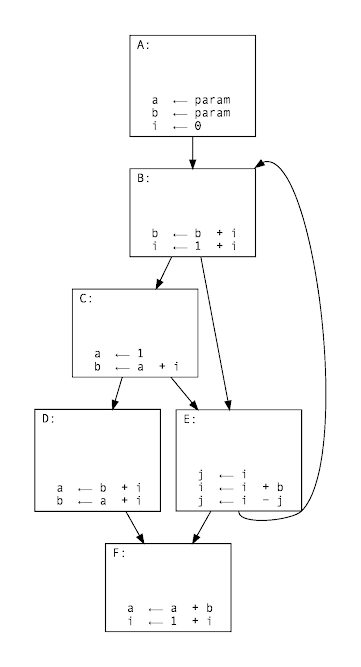
\includegraphics[height=200px]{./cfg.png}
\end{center}
\subsection{Решение}
\label{sec:org87352e3}
Множества \(use_B\) для блоков ГПУ:
\begin{gather*}
use_A = \emptyset \\
use_B = \{ b, i \} \\
use_C = \{ i \}\\
use_D = \{ i, b \}\\
use_E = \{ i, b \}\\
use_F = \{ a, b, i \}
\end{gather*}
Рассчитаем множества \(def_B\), \(Globals\) и \(Blocks\) для разных блоков:
\begin{gather*}
def_A = \emptyset \cup \{ a \} \cup \{ b \} \cup \{ i \} = \{ a, b, i \} \\
def_B = \emptyset \\
def_C = \emptyset \cup \{ a \} \cup \{ b \} = \{ a, b \} \\
def_D = \emptyset \cup \{ a \} = \{ a \} \\
def_E = \emptyset \cup \{ j \} = \{ j \} \\
def_F = \emptyset \\
Globals = \emptyset \cup \{ i \} \cup \{ i \} \cup \{ b, i \} \cup \{ i, b \} \cup \{ a, b, i \} = \{ a, b, i \} \\
Blocks_i = \emptyset \cup \{ B \} \cup \{ C \} \cup \{ D \} \cup \{ E \} \cup \{ F \} = \{ B, C, D, E, F \} \\
Blocks_b = \emptyset \cup \{ B \} \cup \{ D \} \cup \{ E \} \cup \{ F \} = \{ B, D, E, F \} \\
\end{gather*}
Границы доминирования для каждого из блоков:
\begin{gather*}
DF(A) = \emptyset \\
DF(B) = \emptyset \\
DF(C) = \{ E, F \} \\
DF(D) = \{ F \} \\
DF(E) = \{ F \} \\
DF(F) = \emptyset
\end{gather*}
Найдём блоки и переменные, для которых нужно разместить \(\varphi\)-функции:
\begin{enumerate}
\item i:
\begin{itemize}
\item \(WorkList = \{ B, C, D, E, F \}\)
\item \(DF(B) = \emptyset\), так что этот блок пропускается. \(WorkList = \{ C, D, E, F \}\);
\item \(DF(C) = \{ E, F \}\), так что в блоки \(E\) и \(F\) добавляются функции \(\varphi(i, i)\). \(WorkList = \{ D, E, F \}\).
\item \(DF(D) = \{ F \}\), но в блок \(F\) уже добавлена функция \(\varphi(i, i)\), так что ничего не меняется. \(WorkList = \{ E, F \}\).
\item \(DF(E) = \{ F \}\). Аналогично блоку \(D\). \(WorkList = \{ F \}\).
\item \(DF(F) = \emptyset\), так что этот блок пропускается. \(WorkList = \emptyset\), алгоритм завершается.
\end{itemize}
\item b:
\begin{itemize}
\item \(WorkList = \{ B, D, E, F \}\)
\item \(DF(B) = \emptyset\), так что этот блок пропускается. \(WorkList = \{ D, E, F \}\);
\item \(DF(D) = \{ F \}\), так что в блок \(F\) добавляется функция \(\varphi(b, b)\). \(WorkList = \{ E, F \}\).
\item \(DF(E) = \{ F \}\), но в блок \(F\) уже добавлена \(\varphi\)-функция для \(b\), так что ничего не меняется. \(WorkList = \{ F \}\).
\item \(DF(F) = \emptyset\), так что этот блок пропускается. \(WorkList = \emptyset\), алгоритм завершается.
\end{itemize}
\end{enumerate}

Дерево доминаторов для исходного графа:
\begin{center}
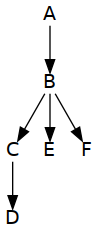
\includegraphics[height=200px]{dom.png}
\end{center}

Перенумеруем переменные:
\begin{enumerate}
\item Блок \(A\) без изменений.
\item В блоке \(B\):
\end{enumerate}
\begin{minted}[]{text}
b_1 = b + i
i_1 = 1 + i
\end{minted}
\begin{enumerate}
\item В блоке \(C\):
\end{enumerate}
\begin{minted}[]{text}
a = 1
b_2 = a + i_1
\end{minted}
\begin{enumerate}
\item В блоке \(D\):
\end{enumerate}
\begin{minted}[]{text}
a_1 = b_2 + i_1
b_3 = a_1 + i_1
\end{minted}
\begin{enumerate}
\item В блоке \(E\):
\end{enumerate}
\begin{minted}[]{text}
i_2 = ϕ(i, i)
j = i_2
i_3 = i_2 - j
\end{minted}
\begin{enumerate}
\item В блоке \(F\):
\end{enumerate}
\begin{minted}[]{text}
i_4 = ϕ(i, i)
b_4 = ϕ(b, b)
a_2 = a_1 + b_3
i_5 = 1 + i_4
\end{minted}
\end{document}
